\begin{frame}{Annotated Circle}
\begin{center}
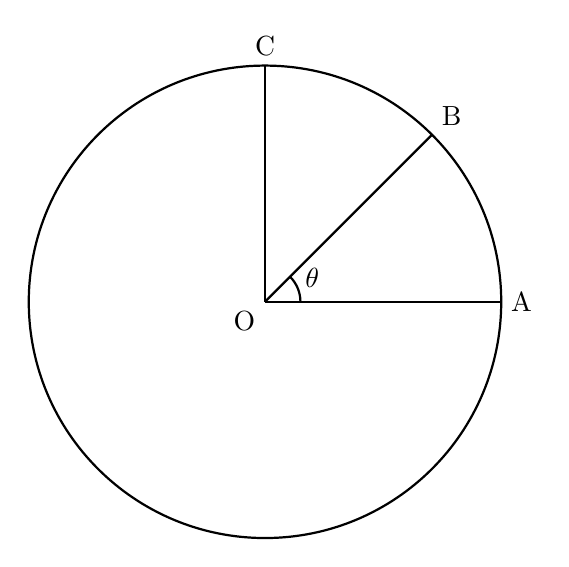
\begin{tikzpicture}[scale=1.5]
    \draw[thick] (0,0) circle (2);
    \draw[thick] (0,0) -- (2,0);
    \draw[thick] (0,0) -- (1.414,1.414);
    \draw[thick] (0,0) -- (0,2);
    
    \node at (0,0) [below left] {O};
    \node at (2,0) [right] {A};
    \node at (1.414,1.414) [above right] {B};
    \node at (0,2) [above] {C};
    
    \draw[thick] (0.3,0) arc (0:45:0.3);
    \node at (0.4,0.2) {$\theta$};
\end{tikzpicture}
\end{center}

\footnotesize
\texttt{\textbackslash draw[thick] (0,0) circle (2);}\\
\texttt{\textbackslash draw[thick] (0.3,0) arc (0:45:0.3);}
\end{frame}